% This is samplepaper.tex, a sample chapter demonstrating the
% LLNCS macro package for Springer Computer Science proceedings;
% Version 2.20 of 2017/10/04
%
\documentclass[runningheads]{llncs}
%
\usepackage{graphicx}
% Used for displaying a sample figure. If possible, figure files should
% be included in EPS format.
%
% If you use the hyperref package, please uncomment the following line
% to display URLs in blue roman font according to Springer's eBook style:
% \renewcommand\UrlFont{\color{blue}\rmfamily}

\begin{document}
%
\title{Anti-Withholding Reward System\\
to Secure Bitcoin Mining Pools}
%
%\titlerunning{Abbreviated paper title}
% If the paper title is too long for the running head, you can set
% an abbreviated paper title here
%
\author{Arijet Sarker\orcidID{0000-1111-2222-3333} \and
Simeon J. Wuthier\orcidID{1111-2222-3333-4444} \and
Sang-Yoon Chang\orcidID{2222--3333-4444-5555}}
%
\authorrunning{Arijet et al.}
% First names are abbreviated in the running head.
% If there are more than two authors, 'et al.' is used.
%
\institute{University of Colorado Colorado Springs \\
\email{\{asarker,swuthier,schang2\}@uccs.edu}
}
%\institute{Princeton University, Princeton NJ 08544, USA \and
%Springer Heidelberg, Tiergartenstr. 17, 69121 Heidelberg, Germany
%\email{lncs@springer.com}\\
%\url{http://www.springer.com/gp/computer-science/lncs} \and
%ABC Institute, Rupert-Karls-University Heidelberg, Heidelberg, Germany\\
%\email{\{abc,lncs\}@uni-heidelberg.de}}
%
\maketitle              % typeset the header of the contribution
%
\begin{abstract}
Miners get reward by solving cryptographic puzzles (mining) in decentralized cryptocurrency system such as Bitcoin. But, the problem with this approach is the high variance of reward for solo miners. Hence, the miners, forming mining pools participate in the mining process to earn more stable reward over time. The reward earned by a mining pool is shared among the participating miners according to their contribution to the pool. But, a number of attacks in the pool make this honest mining less profitable. In Block Withholding (BWH) attack, the attacker joins the victim pool and gets a portion of the pool’s reward unfairly by only pretending to contribute to the victim pool. The Fork After Withholding (FAW) attack is an extension of the BWH attack. In this case, the attacker gets an additional reward by generating intentional fork only when external miners propagate valid blocks. The FAW attacker earns equal to or greater than a BWH attacker. In this paper, a reward system, called Anti-Withholding Reward System (AWRS) is proposed to mitigate the effect of FAW attack as well as BWH attack in the mining pool. The proposed AWRS is designed in such a way that it will discourage the attacker to launch the FAW attack and encourage honest mining. AWRS provides additional incentives to the block submitter by introducing asymmetry between block and shares in the rewards. According to our analyses, AWRS completely disincentives FAW attack and makes the optimal attacker behavior to become honest mining regardless of the attacker's computational power capability. 


\keywords{First keyword  \and Second keyword \and Another keyword.}
\end{abstract}
%
%
%

\section{Introduction}

\subsection{A brief overview}
Since the release of Bitcoin in 2008\cite{b1}, blockchain technology has skyrocketed, and the notion of a distributed consensus has provided the opportunity for new developments that can take out the central authority within a trust-sensitive protocol. By decentralizing an agreement between peers, there is no need to rely on honesty since every user is capable of prove that every piece of the blockchain is valid, thus, leading to a distributed consensus between peers. The consensus protocol is derived from the distributed ledger known as blockchain, which is a permanent linear chain of transactions put into blocks, where every new block is dependent upon the last. Since the blockchain is always increasing in size, the distributed ledger allows all the users in the network to share the same large data structure. Bitcoin, being the most famous blockchain, uses a consensus protocol called proof of work (PoW) which provides a way to mathematically prove that money exists within a user’s account. Within this ledger, BTC tokens are what define Bitcoin as a currency. Since it is a distributed consensus, every peer on the network agrees to the transfer of BTC between accounts. The transactions are put into the blockchain when a block is created, as each new block is capable of carrying a specific size of transactions. The creation of blocks is done through solving a computational puzzle against the rest of the Bitcoin network, thus, those who have a larger computational power have a better chance of solving the puzzle. Once the puzzle is solved, the new block is found and broadcasted to the rest of the network, which updates the computational puzzle for all the miners to restart and search for a new block on top of the newly created one. Miners are incentivized to mine since, upon solving, they are given a transaction that sends them a specific financial reward to that miner’s account. On average, blocks are discovered every ten minutes, known as the blocktime. Because miners are competing against every other miner in the network, solving a block is comparable to winning the lottery. For miners with lower computational power compared to the world, it could take years or decades before the miner discovers a block before anyone else, and receives their first reward. 
% Talk about how although we can estimate the analysis, nothing can be exactly determined since everything is by chance.

Since the PoW protocol relies on computational power, users tend to join in mining pools, where the computation power of the pool is equivalent to summing together every miner’s power. This is an attractive option for miners because the chance of finding a block greatly increases, the reward gets split between each miner in the pool according to each miner’s computational power, thus the frequency of receiving a reward is increased significantly and miners are paid smaller amounts over a long period of time to even out the reward they would have been making from solo-mining.


Since the PoW protocol relies on computational power, users tend to join in mining pools, where the computation power of the pool is equivalent to summing together every miner’s power. This is an attractive option for miners because the chance of finding a block greatly increases, the reward gets split between each miner in the pool according to each miner’s computational power, thus the frequency of receiving a reward is increased significantly and miners are paid smaller amounts over a long period of time to even out the reward they would have been making from solo-mining.

\subsection{Consensus between nodes}
The distributed consensus allows everybody in the network to be anonymous and only visible by their wallet address. Nodes come to an agreement through PoW, which proves that the required computations has been completed, and that the transactions within the solved block are valid and are not withdrawing money that does not exist in an account. Consensus between nodes is determined by the majority of the network that accepts a block as valid, but even then nodes are able to determine if a submitted block is invalid. One of the most known attacks is the 51\% attack which states that when any node in the network achieves a computing power that is greater than 50\%, that node will take the majority of the consensus, and will gain full control over the network by being able to submit and validate invalid transactions. 

\subsection{Blocks}
Each block contains a unique block header, where the hash of this header is used to identify the block. The block header is 80-byte string consisting of a 4-byte Bitcoin version number, 32-byte previous block hash, 32-byte merkle root, 4-byte timestamp, 4-byte difficulty target, and a 4-byte nonce.

The first block in a blockchain is called the genesis block and then every block proceeding it will build on top of the genesis. For a miner to find the next block in the blockchain, the miner needs to hash the block header twice with different nonces to try to find a valid nonce such that the hash of the block header is less than a 256-bit number, $\bar{D}$. This 256-bit number, $\bar{D}$ can be derived from $D=2^{224} \mathbin{/} \bar{D}$ where $D$ is the difficulty number in the Bitcoin network. and is automatically adjusted frequently by the Bitcoin protocol in such a way that it will take roughly %verify the blocktime, or don't include a specific number
10 minutes on average to find a valid block. This is known as the blocktime. Since hashing is a one-way function, the only known way to successfully mine is to guess the correct nonce for the header and then check whether the hash value of the header is below a certain threshold. When a valid block is found, the miner will broadcast their findings to every other node in the Bitcoin network. As previously discussed, if the majority accepts the block as a valid block, then the miner gets the reward of the block. Eventually, every node in the network will update their block to the newly discovered one, and begin the process of searching for a new block again.

\subsection{Pools and Shares}
Since receiving a reward in solo-mining is very rare, grouping together many solo-miners allows the reward to be split between each miner. In this scenario, there needs to be a secure way of determining the computational power of each miner such that the reward for mining a block can be distributed evenly to its users. The pool manager is responsible for ensuring the found block is submitted to the network, and the payment to the users is correct. The method to do this, while still maintaining the security of the decentralized network, is by using shares. Miners search for blocks by guessing a 4-byte nonce and hashing its header twice, if the output is mathematically less than $\bar{D}$, then it can be considered a block, and submitted to the network for a reward. Similarly, the pool manager will select a block difficulty $d$, with $d=2^{224} \mathbin{/} \bar{d}$, where $\bar{d}<\bar{D}$, hence, the block is easier to compute. Any blocks that are mathematically less than $\bar{d}$ but do not qualify as full block, are considered shares. The chance of receiving a share is much greater than the chance of receiving a block. This is important because, it provides a way for the pool manager to measure the computational power of each of its miners, by keeping track of how many shares each miner submits. This is what the pool manager will use to determine the percentage of the pool that a miner is contributing to determine the reward given to each miner. According to \cite{b2}, this is known as the pay per share (PPS) reward scheme.

It is worth noting that each block header is specific to the pool itself, as defined by the block header. When this header gets hashed, all the data becomes permanent on the blockchain, thus, it would be impossible for someone mining in a pool to withhold a block to submit themselves.

%New Section%%%%%%%%%%%%

\section{Preliminaries}
\subsection{Forking}
The blocktime is the average time in which blocks are found within the entire network.If a miner is mining on top of an outdated block, the only way to earn a reward would be to mine more blocks than the main chain. For every new block added on the main chain, there needs to be a greater number of blocks added to the fork, on average. This is unreasonable since that would require more than 50\% of the computing power of the rest of the network. 

When an external miner on the network submits a block, then every miner will end up selecting that block as the main chain. If there are more than one blocks that are broadcasted, then each miner will select the block with the most blocks appended to it. Therefore, when a block is discovered, miners need to broadcast their finding as fast as possible, otherwise another miner may submit a different solution between that time. In Bitcoin, when two miners find and submit valid blocks in relatively the same time, this is considered a fork since the blockchain is then split into multiple paths. The chance that a block has a higher probability of being selected is determined by what majority of the network has already selected that block as the main block. While this solution guarantees only one path will be chosen, it results in a lot of wasted computations, in Bitcoin, the blocks that are not selected as the main chain are considered stale blocks since they have no use to the network. All transactions within a stale block are released back in with the rest of unselected transactions, and all the computing power used to find that block can be considered wasted.
%Depending on the speed at which blocks are found, there is a possibility that two miners on the network will discover a block at roughly the same time, leading to some nodes on the network believing that one block is the most recent, and other nodes believing that another block is the most recent. This is known as a fork, since the blockchain gets split into two paths.

%***** This section mainly provides an in-details description of different bitcoin basic terms such as bitcoin mining, mining pools, fork, role of miners, BWH attack, FAW attack, pay-off-scheme etc.

% !!!! We need to discuss how a block is specific to the miner, so a miner is unable to privately submit a block on their own if they find it in the pool.
% Towards the beginning !!!!!!! need to explain how every miner is anonymous, and spoofing is easy 
% Need to talk about how pools are considered a solo miner, since the pool manager can just spoof their identity to look like just another miner

\subsection{Honest Mining vs. Infiltration Mining}
Infiltration mining is the term used to describe miners that use their resources in an unintended manner, to have control over a piece of the network. Miners have the option to withhold their newly discovered block instead of broadcasting it to the rest of the network for a reward. While withholding a block yields no incentive, it can be used in pools to negatively affect the pool manager.


\subsection{Multiple Forks}
We have analyzed the scenario when two blocks are submitted at relatively the same time. The chance that one block will dominate the other is a 50\% chance. In a situation where more than two miners discover a block, the chance that one miner's block will be selected onto the main chain is $1/n$ where $n$ is the number of branches generated at any given time.

% Preliminaries
%In this section, we describe the process of mining for Bitcoin in depth, and discuss a few of the existing protocols inside of mining pools that attempt to measure the computing power of each miner so that the reward given to the pool can be distributed accordingly.

%\subsection{Blockchain and Mining}
%A blockchain is a permanent linear chain of blocks, where each block depends on the previous block within the chain. It is a distributed consensus system without the need to trust a central authority because it is maintained by every node on the network. The transactions within the blockchain are determined by the majority of the consensus, and any transactions stored within the blockchain can never be modified nor deleted. This is one of the features that allows cryptocurrencies to support money transfer as well as the deployment of contracts between nodes without any root of trust. Transactions are recorded inside a block in the blockchain. Each block contains a limited number of transactions based on the size of the block. Each block also contains a unique block header, where the hash of this header is used to identify the block. The block header is 80-byte string consisting of an 4-byte Bitcoin version number, 32-byte previous block hash, 32-byte merkle root, 4-byte timestamp, 4-byte difficulty target, and a 4-byte nonce. The first block in a blockchain is called the genesis block and then every block proceeding it will build on top of the genesis. Miners are paid by searching for the next valid block in the blockchain. In order to do that, the miners hash the block header twice with different nonces to try to find a valid nonce such that the hash of the block header is less than a 256-bit number, $\bar{D}$. This 256-bit number, $\bar{D}$ can be derived from $D=2^{224} \mathbin{/} \bar{D}$ where $D$ is the difficulty number in the Bitcoin network. and is automatically adjusted frequently by the Bitcoin protocol in such a way that it will take roughly 10 minutes on average to find a valid block. This is known as the blocktime. Since hashing is a one-way function, the only known way to successfully mine is to guess the correct nonce for the header and then check whether the hash value of the header is below a certain threshold. When a valid block is found, the miner will broadcast their findings to every other node in the Bitcoin network. If the majority accepts the block as a valid block, then the miner gets the reward of the block. Eventually, every node in the network will update their block to the newly discovered one, and begin the process of searching for a new block again.

%\subsection{Mining Pools}
%Since receiving a reward in solo-mining is very rare, grouping together many solo-miners allows the reward to be split between each miner. In this scenario, there needs to be a secure way of determining the computational power of each miner such that the reward for mining a block can be distributed evenly to its users. The pool manager is responsible for ensuring the found block is submitted to the network, and the payment to the users is correct. The method to do this, while still maintaining the security of the decentralized network, is by using shares. Miners search for blocks by guessing a 4-byte nonce and hashing its header twice, if the output is mathematically less than $\bar{D}$, then it can be considered a block, and submitted to the network for a reward. Similarly, the pool manager will select a block difficulty $d$, with $d=2^{224} \mathbin{/} \bar{d}$, where $\bar{d}<\bar{D}$, hence, the block is easier to compute. Any blocks that are mathematically less than $\bar{d}$ but do not qualify as full block, are considered shares. The chance of receiving a share is much greater than the chance of receiving a block. This is important because, it provides a way for the pool manager to measure the computational power of each of its miners, by keeping track of how many shares each miner submits. This is what the pool manager will use to determine the percentage of the pool that a miner is contributing to determine the reward given to each miner. According to [Rosenfeld's paper!!!!!!!!!!!!!!], this is known as the pay per share (PPS) reward scheme.

%It is worth noting that each block header is specific to the pool itself, as defined by the block header. When this header gets hashed, all the data becomes permanent on the blockchain, thus, it would be impossible for someone mining in a pool to withhold a block to submit themselves.

%\subsection{Forks}
%When an external miner (somewhere in the network) submits a block, every miner selects the block that is most recent. If there are more than one blocks that are broadcasted, then each miner will select the block with the most blocks appended to it. Therefore, when a block is discovered, the miner needs to broadcast it as fast as possible, otherwise another miner may submit a different solution between that time. In Bitcoin, when two miners find and submit valid blocks in relatively the same time, this is considered a fork since the blockchain is then split into multiple paths. The chance that a block has a higher probability of being selected is determined by what majority of the network has already selected that block as the main block. While this solution guarantees only one path will be chosen, it results in a lot of wasted computations, in Bitcoin, the blocks that are not selected as the main chain are considered stale blocks since they have no use to the network.  

%Depending on the speed at which blocks are found, there is a possibility that two miners on the network will discover a block at roughly the same time, leading to some nodes on the network believing that one block is the most recent, and other nodes believing that another block is the most recent. This is known as a fork, since the blockchain gets split into two paths.

%***** This section mainly provides an in-details description of different bitcoin basic terms such as bitcoin mining, mining pools, fork, role of miners, BWH attack, FAW attack, pay-off-scheme etc.

% !!!! We need to discuss how a block is specific to the miner, so a miner is unable to privately submit a block on their own if they find it in the pool.
% Towards the beginning !!!!!!! need to explain how every miner is anonymous, and spoofing is easy 
% Need to talk about how pools are considered a solo miner, since the pool manager can just spoof their identity to look like just another miner

\section{Literature Review}
\subsection{Block Withholding Attacks}
An advanced miner is capable of partitioning a portion of their computational power to infiltration mining. In this scenario, when the miner finds a share through infiltration mining on another pool, they will submit it to show that pool manager that they are helping in the search for a block. This miner will reap the benefits from another pool, however, if this miner discovers a full block through infiltration mining then they should not submit it until another user in the world broadcasts that they have found also a block. By doing this, the pool manager will buy themselves more time for solo-mining, while also bringing the chance that the fork they created will become a stale block. This is known as Fork After Withholding (FAW) and the equation is as follows:
%Fix formatting
\begin{eqnarray}
R_{FAW}=\frac{\alpha  (1-\tau )}{1-\alpha  \tau }+\frac{(\alpha  \tau ) \left(\frac{\beta }{1-\alpha  \tau }+\frac{\alpha  c \tau  (-\alpha -\beta +1)}{1-\alpha  \tau }\right)}{\alpha  \tau +\beta }
\end{eqnarray}

\section{Our Proposal}
\subsection{Detection}
Detecting an FAW attack requires the pool manager to have knowledge of the attacker's computing power. When a block is submitted to the pool manager, the manager can check if an external block was also submitted, if that is the case, then the pool manager has the possibility of an infiltration miner. Since the pool manager has this miner's address, he can blacklist the attacker, however, this would not work very well since the blockchain is anonymous and the attacker can just as easily spoof a new address and infiltration mine from there. The pool manager has no way of being certain that he is being attacked, however, by simply analyzing the time between an external miner's broadcast and an internal miner's broadcast to the pool manager, the pool manager can partially determine if he has infiltration miners.

The victim pool manager can only see $\tau \alpha$, i.e. the computing power of the attacker's infiltration mining. But since $\tau$ and $\alpha$ cannot be separated, the pool manager can assume the worst case for his pool, where $\tau=\hat{\tau}$,  in the case where the attacker's infiltration mining is optimized to receive the greatest reward. 

While the attacker is able to control $\tau$, we propose the pool manager be able to control the special reward given to the block solver, which will be different from different from the other miner's rewards within the pool. The reward given to the block solver can be denoted as $\Gamma$ which will have domain of $0\leq\Gamma\leq1$. When $\Gamma=0$ will give no reward to the block solver. This can be considered the same as block withholding. When $\Gamma=1$, the attacker will receive the reward of the entire pool. This can be considered the same as solo-mining, since nobody else in the pool will receive a reward. The equation changes to
% Fix formatting
\begin{eqnarray}
R_{AWRS}=\frac{\beta  (1-\Gamma ) (\alpha  \tau )}{(1-\alpha  \tau ) (\alpha  \tau +\beta )}+\frac{\alpha  (1-\tau )}{1-\alpha  \tau }+\frac{\alpha  c \tau  (-\alpha -\beta +1) \left(\frac{(\alpha  \tau ) (1-\Gamma )}{\alpha  \tau +\beta }+\Gamma \right)}{1-\alpha  \tau }
\end{eqnarray}

Similar to the FAW payment, ...
%***** In this section, we will provide details mathematical analysis with technical terms to discuss the reward gain of an attacker. We can multiple pools scenarios too.

\section{Defense Mechanism / Countermeasures / Proposed Solution}
Since $R_{HONEST}=\alpha$, when $R_{AWRS}>\alpha$, there is incentive to infiltration mine is greater than honest mining. To mitigate the FAW attack, the pool manager is able to control $\Gamma$. The optimal value for $\Gamma$ is one where $R_{AWRS}\leq\alpha$, i.e. the pool manager would need to select a break-even value such that the reward will always be less than or equal to honest mining. The equation to show this is as follows
\begin{eqnarray}
\Gamma_{BE}=\frac{\alpha(\beta+(\alpha-1-c\tau(\alpha+\beta-1)))}{\beta+c\beta(\alpha+\beta-1)}
\end{eqnarray}
 But since $\Gamma_{BE}$ contains $\tau$, the solution is ambiguous since it is dependent upon whatever proportion the attacker dedicates to infiltration mining. Assuming that an attacker will choose $\tau=\hat{\tau}$ to maximize their reward, the pool manager is able to assume the worst-case and change $\Gamma$ accordingly.
\begin{eqnarray}
\hat{\tau}=\frac{\sqrt{-\alpha ^2 \beta ^2 (c (\alpha +\beta -1) (\Gamma -1)+\Gamma -1) (-\alpha  (\beta +1)+\beta  \Gamma +c (\alpha +\beta -1) (\beta \Gamma +1)+1)}+\alpha  \beta  (\alpha -c (\alpha +\beta -1)-1)}{\alpha ^2 (-\alpha +\beta  (\Gamma -1)+c (\alpha +\beta -1) (\beta  (\Gamma -1)+1)+1)}
\end{eqnarray}
!!! Explain that we need to assume $\tau$ is zero instead

By plugging in $\tau=0$ to become $\hat{\Gamma}_{BE}$, we get
\begin{eqnarray}
\hat{\Gamma}_{BE}=\frac{\alpha }{c (\alpha +\beta -1)+1}
\end{eqnarray}
By plugging $\hat{\Gamma}_{BE}$ into $R_{AWRS}$, the reward is altered to ensure that, regardless of $\tau$, $\hat{R}_{AWRS}\leq\alpha$, the reward becomes
\begin{eqnarray}
\hat{R}_{AWRS}=\frac{\alpha  \left(\alpha  (\beta -1) \tau -\beta +\alpha  \tau ^2 (c (\alpha +\beta -1)+1)\right)}{(\alpha  \tau -1) (\alpha  \tau +\beta )}
\end{eqnarray}
Now, when $\tau>0$ inside $\hat{R}_{AWRS}$, the reward will always be less than honest mining. When $\tau=0$, the reward will be equal to honest mining. Since this is still an ambiguous solution, the pool manager can assume $\tau=\hat{\tau}$ where $\hat{\tau}=0$, so
\begin{eqnarray}
\hat{R}_{AWRS}=0
\end{eqnarray}
\section{Analysis Using Simulation}

Here, we show the behavior of our payment equation compared to that of FAW, and honest mining.

%***** Here, we will show our graphs and simulations to provide the proofs of our argument.

%\begin{figure}[h!]
%  \includegraphics[width=\linewidth]{images/alphavsoptimaltau.png}
%  \label{fig:alphavsoptimaltau}
%\end{figure}
%Figure \ref{fig:alphavsoptimaltau} shows how $\hat{\tau}$ increases as the attacker's computing power ($\alpha$) increases. for different mining pool powers ($\beta$).
%\begin{figure}[h!]
%  \includegraphics[width=\linewidth]{images/alphavsbreakevenGamma.png}
%  \label{fig:alphavsbreakevenGamma}
%\end{figure}

%In figure \ref{fig:alphavsbreakevenGamma} break-even Gamma ($\Gamma_{BE}$) is analyzed for different values of $\alpha$ and $\beta$.
%\begin{figure}[h!]
%  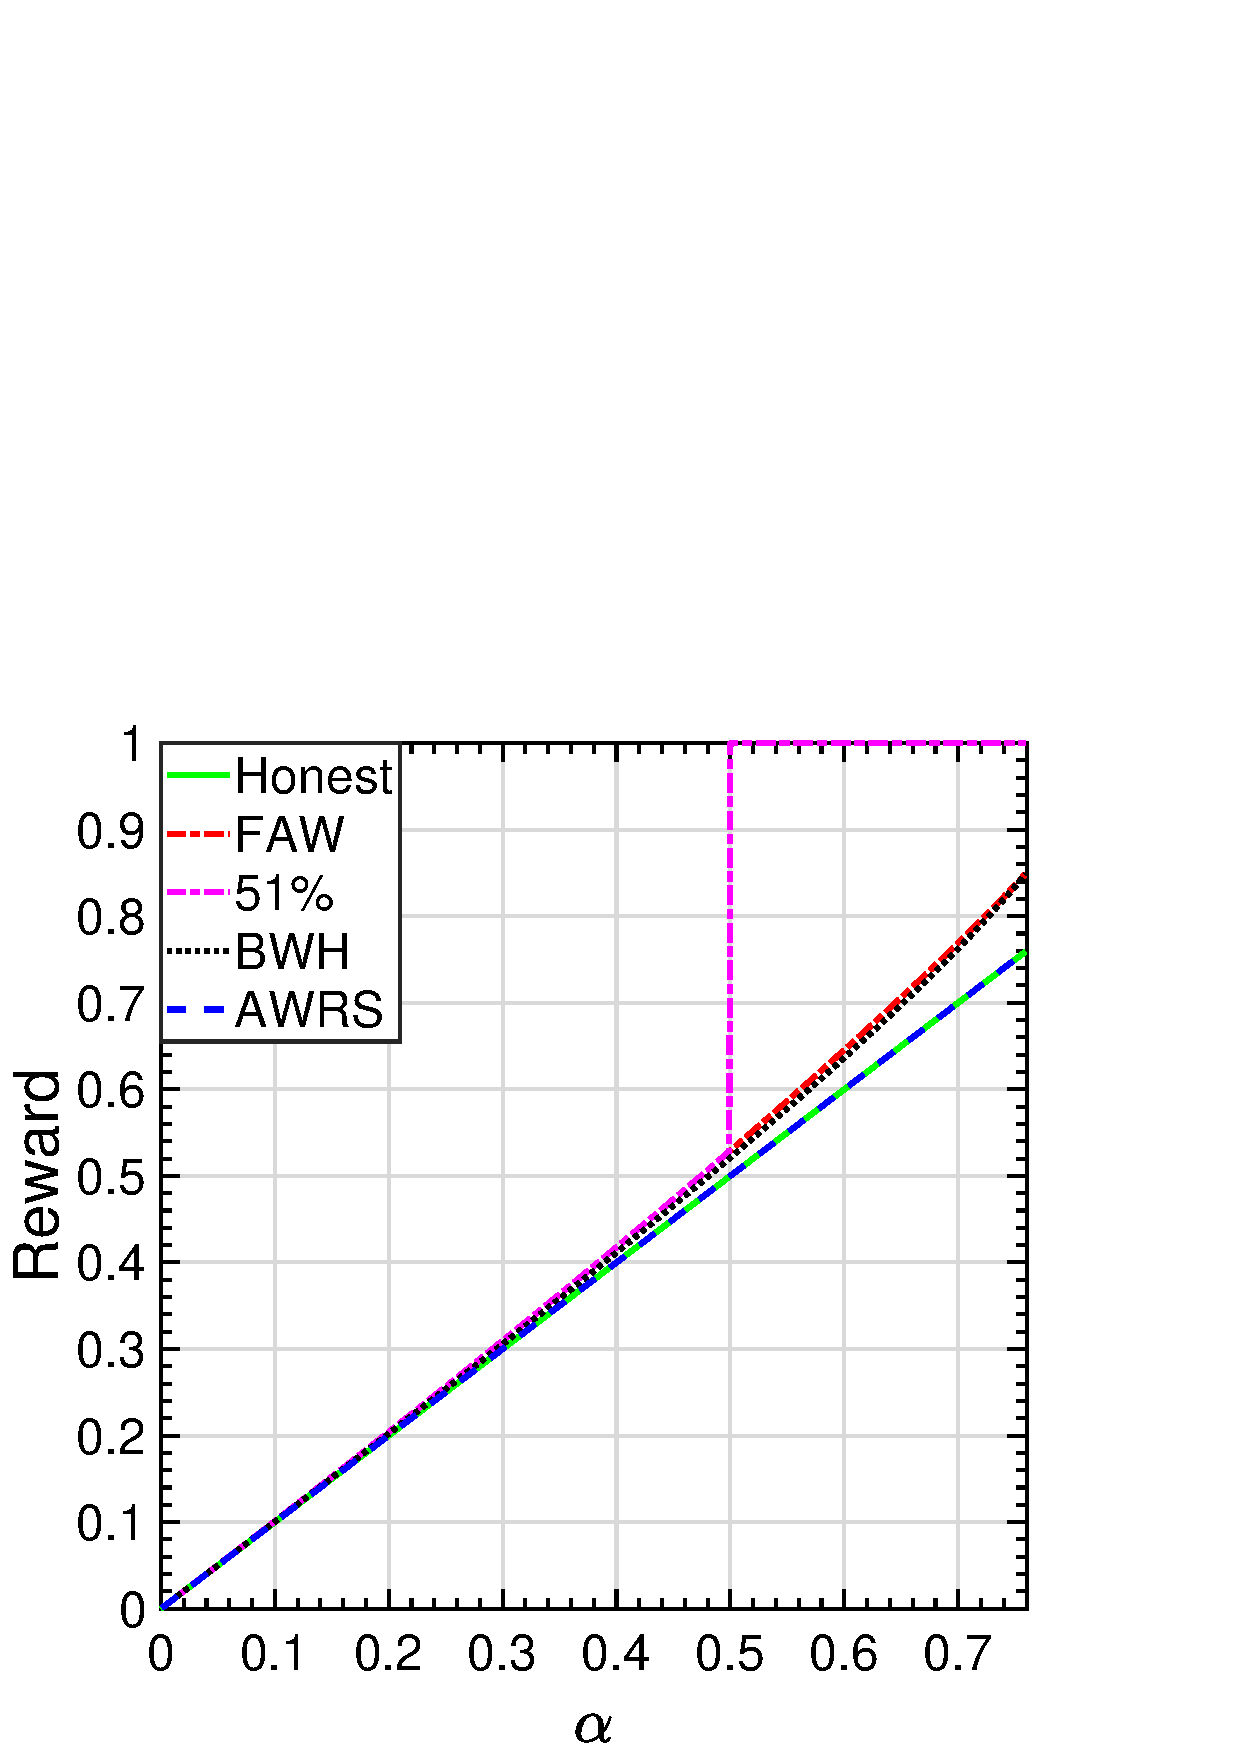
\includegraphics[width=\linewidth]{images/alphavsreward.png}
%  \label{fig:alphavsreward}
%\end{figure}

In reality, it is not possible for the pool manager to know the computational power of the attacker (alpha) exactly and how much computational power (tau) is used by the attacker as an infiltration mining ($\tau\alpha$). However, if $\alpha$ increases, then $\hat{\tau}$ also increases or, at least remains same for value of c up to 0.76 (see the graph $\alpha$ vs $\hat{\tau}$). If alpha increases, then $\Gamma_{BE}$ also increases (see the graph alpha vs break-even Gamma).
Now, considering the miner with highest computational power in the pool as the attacker, the pool manager can better estimate the value of break-even Gamma value in the AWRS equation.

$\hat{\tau}\alpha$ is miner with highest computational power in the pool

Now, by guessing $\alpha$, the mining pool manager can use the public information of computational power of different mining pools.

miner with highest computational power in the pool is also known by the mining pool manager.

So, from this information, he can calculate the $\hat{\tau}$ value. Thus, he can also calculate the break-even Gamma for the miner with highest computational power in the pool. This calculation may not have been exactly accurate, but it can give an idea of alpha, optimal tau to the pool manager. Thus, he can have a better estimation of break-even Gamma.

If he sets this value as the Gamma value in the AWRS equation, then it is highly likely that all the miners have to do the honest mining.   


\section{Offense and Defense}
\subsection{Optimal Attacker Strategy}

%~\ref{XXXX}
As discussed in the threat model in Section[!!!!!!!!!!], we assume the worst-case scenario from an attacker, and give the attacker the capability to dynamically adapt its control parameter $\tau$ to maximize its reward for conducting the FAW attack, i.e. the attacker solves the following optimization problem where $R$ is the attacker reward against AWRS: 

$\mbox{max}_{\tau} R_{\Gamma=0,\gamma=1}$
Solving the optimization problem yields the FAW-optimal tau ($\hat{\tau}$): 

$\hat{\tau}  =  \mbox{argmax}_{\tau} R_{\Gamma=0,\gamma=1}$

%& = &                              % SYC: tau-hat equation (solving dR/dtau = 0)





\subsection{Defense Control Parameters}


In contrast to the attacker maximizing its unfair reward advantage, the mining pool manager aims to minimize the attacker's reward. This can be done by assuming the attacker is setting $\tau=\hat{\tau}$.

The block reward distribution is a zero-sum game, so reducing the attacker's reward discourages the attacker from conducting block-withholding/FAW attacks and increases the fairness among the miners. 

We first explain the $(\Gamma,\gamma)$-strategy minimizing the attacker reward ($(\hat{\Gamma},\hat{\gamma})$) and then explain our choice of the break-even strategy ($(\Gamma_{\mbox{BE}},\gamma_{\mbox{BE}})$) which uses small $\Gamma$ than $\hat{\Gamma}$ (to reduce the mining variance, e.g., $\Gamma=1$ is equivalent to solo mining). 


%~\ref{XXXY}
The mining pool manager's control parameter $\Gamma$ is designed to discourage withholding-based attacks, and increasing $\Gamma$ decreases the attacker reward, as shown in Figure[!!!!!!!!!!!]. 

To find the optimal $\Gamma$ and $\gamma$ ($(\hat{\Gamma},\hat{\gamma})$), we solve the following optimization problem: 



%SYC: Explain Gamma-hat using the min-max optimization, which minimizes the reward with respect to $(\Gamma,\gamma)$ after the attacker maximized the FAW-reward with respect to $\tau$ first, similarly to the optimal \tau explanation in the optimal-attacker section



% SYC: Plot Gamma-hat with respect to gamma-hat and explain it



However, the mining pool manager choosing $(\Gamma,\gamma) = (\hat{\Gamma},\hat{\gamma})$ can be too constraining and, more importantly, irrelevant. 

The attacker can simply toggle to the honest-mining strategy if $R < \alpha$, as discussed in the threat model in Section%~\ref{XXXX}
, making the optimization effort meaningless beyond making the attacker reward converge towards an honest-mining reward, i.e., $R \rightarrow \alpha$. 

Therefore, AWRS uses the \emph{break-even ($\Gamma,\gamma)$} ($\Gamma_{BE},\gamma_{BE}$) solving $R = \alpha$. 

Given $\alpha$, $\beta$, $c$, and $\tau = \hat{\tau}$, AWRS uses the following for its defense:
\begin{equation}
\Gamma=\frac{ \alpha(\beta+(-1+\alpha-c(\alpha+\beta-1))\hat{\tau}}{ \beta+c\beta(\alpha+\beta-1)\gamma}
\end{equation}
%$Γ = (α*(β+(-1+α-c*(α+β-1))*τ_hat))/(β+c*β*(α+β-1)*γ)$      % SYC: Need in Latex
%   =                  % SYC: Plug in the $\hat{\tau}$ expression so get rid of $\tau$
We set $\tau=\hat{\tau}$ to get a reward that is not dependent upon $\tau$, because we will assume the worst case where the attacker maximizes their reward.

!!!

As is seen in Equation %~\ref{XXYY}
, choosing $\Gamma$ in such a way that is independent  $\tau$ assuming that the attacker chooses $\hat{\tau}$ to optimize their reward from the FAW attack%~\cite{XYYY_FAW_paper}. 
i.e. the mining pool manager needs to estimate the parameters given by the mining environment but not the control parameter of the attacker; 

the mining pool manager aims to mitigate the worst-case FAW attack. 


By Kerckhoff's principle, if the attacker knows the mining pool manager's defense strategies, including the choice of $\Gamma$ and $\gamma$, then it can choose to adapt the $\tau$ even further to adjust to the defense and choose $\tau = \hat{\hat{\tau}}$ to increase the reward. 

Even if the mining pool manager cannot adapt to such attacker adaptation (providing the attacker greater capability than the defender in the mining pool manager), AWRS is still robust to such attacker adaptation. 



% SYC: Plot Gamma-BE and gamma-BE and explain it.




% SYC: Plot the reward difference between \tau=\hat{\hat{\tau}} and \alpha (the \tau=\hat{\tau} case)

The attacker reward has very small advantage over honest mining in these cases, and AWRS significantly mitigates the withholding-based attacks, the state of the art being the FAW attack. 



\subsection{Better Estimation of Break-Even Gamma in the Real World}
Another solution to estimate $\Gamma_{BE}$ would be to ...



\section{Conclusion}

%\begin{multicols}{2}
%    \begin{equation}
%        I(pair_1,pair_2)=
%        \begin{cases}
%            0 & \text{if }
%            \begin{cases}
               % \max\left(r\left(pair_1^{rx}\right),r\left(pair_2^{tx}\right)\right)\leq d(pair_1^{rx},pair_2^{tx}) \\
                \& \\
               % \max\left(r\left(pair_1^{tx}\right),r\left(pair_2^{rx}\right)\right)\leq d(pair_1^{tx},pair_2^{rx})
%            \end{cases}\\
%            1 & \text{otherwise}
%        \end{cases}
%    \end{equation}
%\end{multicols}

We have shown how our equation can be used to remove the incentive from the FAW attack. By assuming an attacker within the pool is

%\lipsum[10]\lipsum[9]\lipsum[8]\lipsum[7]\lipsum[6]\lipsum[5]\lipsum[4%]\lipsum[3]\lipsum[2]\lipsum[10]\lipsum[9]\lipsum[8]

\section*{Acknowledgment}

%
%bibliographystyle{ACM-Reference-Format}
%\buibliography{../All}
%

\begin{thebibliography}{00}
\bibitem{b1} Satishi Nakamoto. ``Bitcoin: A peer-to-peer electronic cash system," 2008.
\bibitem{b2} M. Rosenfeld, ``Analysis of bitcoin pooled mining reward
systems,” CoRR, vol. abs/1112.4980, 2011. [Online]. Available:
http://arxiv.org/abs/1112.4980
%\bibitem{b2} J. Clerk Maxwell, A Treatise on Electricity and Magnetism, 3rd ed., vol. 2. Oxford: Clarendon, 1892, pp.68--73.
%\bibitem{b3} I. S. Jacobs and C. P. Bean, ``Fine particles, thin films and exchange anisotropy,'' in Magnetism, vol. III, G. T. Rado and H. Suhl, Eds. New York: Academic, 1963, pp. 271--350.
%\bibitem{b4} K. Elissa, ``Title of paper if known,'' unpublished.
%\bibitem{b5} R. Nicole, ``Title of paper with only first word capitalized,'' J. Name Stand. Abbrev., in press.
%\bibitem{b6} Y. Yorozu, M. Hirano, K. Oka, and Y. Tagawa, ``Electron spectroscopy studies on magneto-optical media and plastic substrate interface,'' IEEE Transl. J. Magn. Japan, vol. 2, pp. 740--741, August 1987 [Digests 9th Annual Conf. Magnetics Japan, p. 301, 1982].
%\bibitem{b7} M. Young, The Technical Writer's Handbook. Mill Valley, CA: University Science, 1989.
\end{thebibliography}

\section{Analysis and Simulation}
Considering the FAW attack in the mining pool as a game, the attacker’s strategy is to maximize his reward using less resource and the pool manager’s strategy is to distribute the earned reward among the miners in the pool according to their computational power. In fact, this is a zero-sum game, where the gain or loss of the attacker will directly affect the gain or loss of the miners in the pool and vice versa. Since, the miners are opportunistic, reward variance is the sole deciding factor for them to join or leave a mining pool. \\

The reward maximization of the FAW attacker depends on the computational power of the attacker ($\alpha$), size of the victim pool ($\beta$), the amount of mining power used as infiltration mining ($\tau$) and probability that an attacker’s FPoW through infiltration mining will be selected as main chain (c). However, the attacker can always earn more reward than honest mining regardless of the value of c and the size of the victim pool, $\beta$ (Ref: FAW paper). On the other hand, the reward of the attacker is always an increasing function of the computational power of the attacker and the size of the victim pool, given that the proper $\tau$ is chosen. Considering this, it is always beneficial for the attacker to attack the large pool, as the size of the pool increases, the reward also increases. The reward of the attacker is also an increasing function of c.  \\


However, this is not the case for infiltration mining power, $\tau$. If $\tau$ increases, then the reward of the attacker will begin to increase or, remain constant up to a certain value of $\tau$ and after that it will begin to decrease. Therefore, it is important for the attacker to calculate the optimal value of $\tau$, for which the reward of the attacker will be maximized. Since the FAW attack is always more profitable than honest mining, the attacker will want to use more of his mining power as optimal infiltration mining power to maximize his reward. Therefore, the attacker will target more powerful victim pool, as it will let him the chance of using more optimal infiltration mining power. However, this is valid for the value of c up to 0.76. 

Unless otherwise stated, we have assumed that, $\beta$ = 0.24, c = 0.5 and $ 0 < $ $\alpha$ $+$ $\beta$ $< 1$
%$0$ < $\alpha$ + $\beta$ < $1$




\appendix
\section{\\Title of Appendix A}
***** Here, we will show our calculation of gamma, Gamma for R sub FAW=alpha, R sub FAW less than alpha, optimal tau, etc.
\end{document}


\section{First Section}
\subsection{A Subsection Sample}
Please note that the first paragraph of a section or subsection is
not indented. The first paragraph that follows a table, figure,
equation etc. does not need an indent, either.

Subsequent paragraphs, however, are indented.

\subsubsection{Sample Heading (Third Level)} Only two levels of
headings should be numbered. Lower level headings remain unnumbered;
they are formatted as run-in headings.

\paragraph{Sample Heading (Fourth Level)}
The contribution should contain no more than four levels of
headings. Table~\ref{tab1} gives a summary of all heading levels.

\begin{table}
\caption{Table captions should be placed above the
tables.}\label{tab1}
\begin{tabular}{|l|l|l|}
\hline
Heading level &  Example & Font size and style\\
\hline
Title (centered) &  {\Large\bfseries Lecture Notes} & 14 point, bold\\
1st-level heading &  {\large\bfseries 1 Introduction} & 12 point, bold\\
2nd-level heading & {\bfseries 2.1 Printing Area} & 10 point, bold\\
3rd-level heading & {\bfseries Run-in Heading in Bold.} Text follows & 10 point, bold\\
4th-level heading & {\itshape Lowest Level Heading.} Text follows & 10 point, italic\\
\hline
\end{tabular}
\end{table}


\noindent Displayed equations are centered and set on a separate
line.
\begin{equation}
x + y = z
\end{equation}
Please try to avoid rasterized images for line-art diagrams and
schemas. Whenever possible, use vector graphics instead (see
Fig.~\ref{fig1}).

\begin{figure}
\includegraphics[width=\textwidth]{fig1.eps}
\caption{A figure caption is always placed below the illustration.
Please note that short captions are centered, while long ones are
justified by the macro package automatically.} \label{fig1}
\end{figure}

\begin{theorem}
This is a sample theorem. The run-in heading is set in bold, while
the following text appears in italics. Definitions, lemmas,
propositions, and corollaries are styled the same way.
\end{theorem}
%
% the environments 'definition', 'lemma', 'proposition', 'corollary',
% 'remark', and 'example' are defined in the LLNCS documentclass as well.
%
\begin{proof}
Proofs, examples, and remarks have the initial word in italics,
while the following text appears in normal font.
\end{proof}
For citations of references, we prefer the use of square brackets
and consecutive numbers. Citations using labels or the author/year
convention are also acceptable. The following bibliography provides
a sample reference list with entries for journal
articles~\cite{ref_article1}, an LNCS chapter~\cite{ref_lncs1}, a
book~\cite{ref_book1}, proceedings without editors~\cite{ref_proc1},
and a homepage~\cite{ref_url1}. Multiple citations are grouped
\cite{ref_article1,ref_lncs1,ref_book1},
\cite{ref_article1,ref_book1,ref_proc1,ref_url1}.
%
% ---- Bibliography ----
%
% BibTeX users should specify bibliography style 'splncs04'.
% References will then be sorted and formatted in the correct style.
%
% \bibliographystyle{splncs04}
% \bibliography{mybibliography}
%
\begin{thebibliography}{8}
\bibitem{ref_article1}
Author, F.: Article title. Journal \textbf{2}(5), 99--110 (2016)

\bibitem{ref_lncs1}
Author, F., Author, S.: Title of a proceedings paper. In: Editor,
F., Editor, S. (eds.) CONFERENCE 2016, LNCS, vol. 9999, pp. 1--13.
Springer, Heidelberg (2016). \doi{10.10007/1234567890}

\bibitem{ref_book1}
Author, F., Author, S., Author, T.: Book title. 2nd edn. Publisher,
Location (1999)

\bibitem{ref_proc1}
Author, A.-B.: Contribution title. In: 9th International Proceedings
on Proceedings, pp. 1--2. Publisher, Location (2010)

\bibitem{ref_url1}
LNCS Homepage, \url{http://www.springer.com/lncs}. Last accessed 4
Oct 2017
\end{thebibliography}
\end{document}
